\chapter{Geometric Parameters}

\section{Wing Basic Geometric Parameters}

\begin{figure}
  \centering
  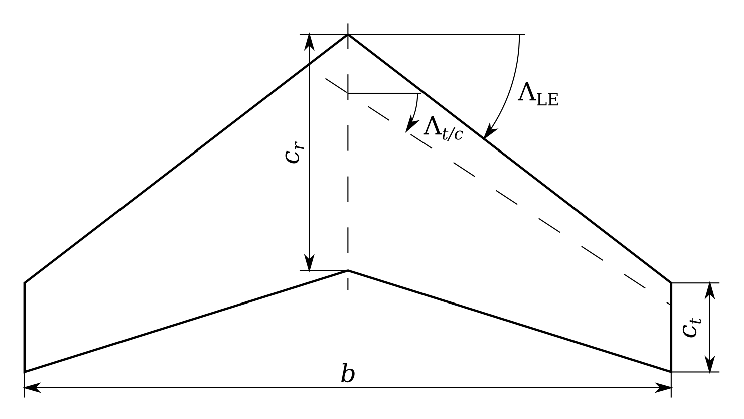
\includegraphics[width=120mm]{images/wing_geometric_parameters.eps}
  \caption{Wing basic geometric parameters}
\end{figure}

Aspect ratio is given by the following formula: \cite{Raymer1992}
\begin{equation}
  A = \frac{b^2}{S}
\end{equation}

Taper ratio is given by the following formula. \cite{Raymer1992}
\begin{equation}
  \lambda = \frac{c_t}{c_r}
\end{equation}

\section{Mean Aerodynamic Chord}

\begin{figure}
  \centering
  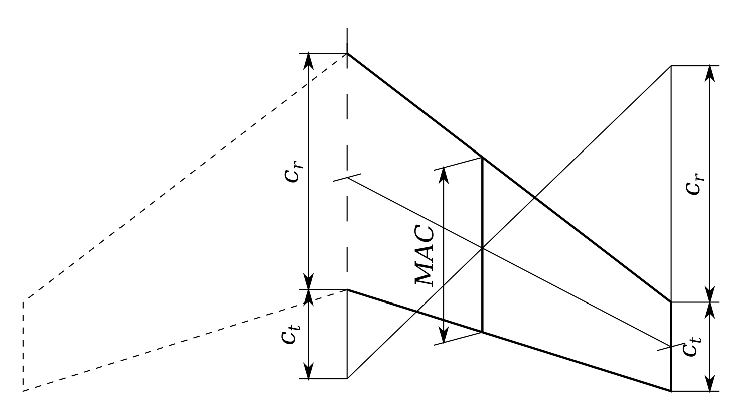
\includegraphics[width=120mm]{images/wing_mean_aerodynamic_chord.eps}
  \caption{Mean aerodynamic chord}
\end{figure}

For tapper wing mean aerodynamic chord can be calculated using following formula: \cite{Corke2003, Galinski2016}
\begin{equation}
  \hat c = \frac{2}{3} c_r \frac{1+\lambda+\lambda^2}{1+\lambda}
\end{equation}

For more complex shapes mean aerodynamic chord is given as follows: \cite{Paturski02}
\begin{equation}
  \hat c = 
  \left(
    \int_{-\frac{b}{2}}^{\frac{b}{2}} \left( c \left( y \right) \right)^2 dy
  \right)
  \div
  \left(
    \int_{-\frac{b}{2}}^{\frac{b}{2}} \left( c \left( y \right) \right) dy
  \right)
\end{equation}

\section{Wing Aerodynamic Center}

\begin{figure}
  \centering
  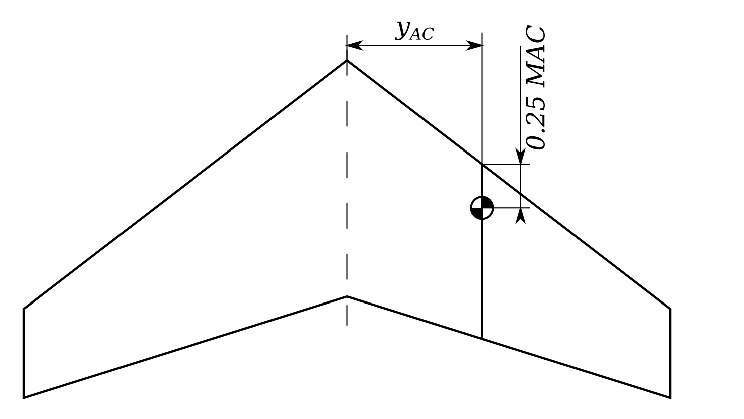
\includegraphics[width=120mm]{images/wing_aerodynamic_center.eps}
  \caption{Wing aerodynamic center}
\end{figure}

Position of wing aerodynamic center ${\vec r}_{AC}$ is at 25\% of the mean aerodynamic chord and its lateral coordinate is given by the following formula. \cite{Raymer1992, Corke2003, Galinski2016, Torenbeek1982}
\begin{equation}
  y_{AC} =
  \frac{ b \left( 1 + 2 \lambda \right) }{ 6 \left( 1 + \lambda \right) }
\end{equation}
